In this section, we present \name{}, an extensible software framework to run observability experiments\footnote{\url{https://github.com/nymphbox/oxn}}. 
\name{} follows the design principles for cloud benchmarking \cite{Silva_CloudBench_2013,2017-Bermbach-Book-CloudServiceBenchmarking,Bermbach_Benchfoundry_2017} and thus particularly strives for portable, repeatable, and relevant experiments.
We built \name{} around a \textsc{yaml}-based configuration file that allows experiments to be shared, versioned and repeated. 
The experiment configuration describes the SUE, i.e., deployment, treatments, workload and response variables  to collect (see \cref{sec:experiments}). 
Using this single experiment file \name{} orchestrates the complete experiment (see~\Cref{fig:oxn-architecture}), by first building and deploying the SUE as well as the load-generator. We use an extendable \textit{runner} component to execute different treatments, such as killing a service container, in combination with the automatic collection of experiment response variables through an observer component. 
For that, we partly rely on the SUE to implement the \textsc{OpenTelemetry} standard, with tools from the CNCF stack\footnote{\url{https://landscape.cncf.io}}, namely \textsc{Jaeger} and \textsc{Prometheus}. 

\begin{figure}[b]
    \centering
    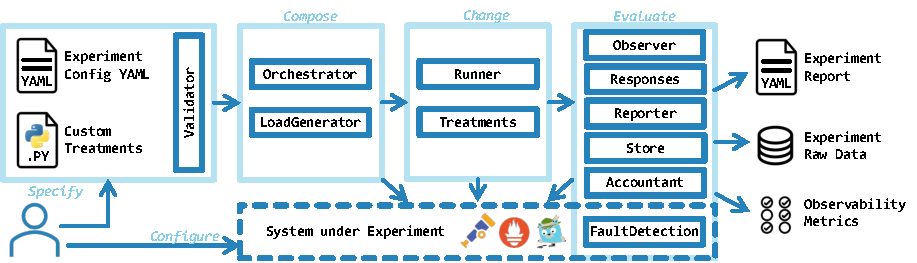
\includegraphics[width=\columnwidth]{figures/oxn_10.pdf}
    \caption{System architecture of \name{}}
    \label{fig:oxn-architecture}
\end{figure}

\subsection{Architecture}
The design of \name{} is modular, decoupled, and extensible. 
At its core, \name{} combines an \textit{orchestrator} to manage the SUE, a \textit{runner} to enact treatments, a \textit{load generator} to stress the SUE and \textit{observers} to capture results.
These components all use existing, well-tested software, which we loosely coupled together to enable observability experiments. Thus, each can be replaced or extended to adapt to different SUE or treatments.
For example, we used \textsc{Docker Compose} for the orchestrator. However, we could have also used a \textsc{Kubernetes}-based orchestrator or one based on \textsc{CloudFormation}. 
For the runner, we rely on an \textsc{Python} interface that can be used to manipulate the SUE.
For the load generator, we use the \textsc{Locust} framework, and for the observers, we implemented interfaces to query \textsc{Jaeger} and \textsc{Prometheus} for now.

Fault and instrumentation \textit{treatments} are defined in a flexible treatment model. %
\Cref{table:fault-treatment-library} shows the fault and instrumentation treatments implemented in our prototype. In addition to these treatments, custom treatments can be added easily by implementing a new treatment class against our treatment interface. This allows
\name{} to be extended with arbitrary fault scenarios or with new instrumentation approaches. Thus, allowing practitioners to build up a large library of relevant faults and treatments to test with \name{}.
\begin{table}[t]
    \caption{Different treatments implemented in \textsc{oxn}} \label{table:instrumentation-treatment-library}\label{table:fault-treatment-library}
    \resizebox{\columnwidth}{!}{\newcounter{treatmentsFoodnoteCounter}
\setcounter{treatmentsFoodnoteCounter}{\value{footnote}} \centering
\newcommand{\rightIndent}{\hspace{0.2cm}}
\begin{tabular}{lp{0.6\columnwidth}l}
    Name & Purpose & Tool \\ \hline
    \multicolumn{3}{l}{\textbf{Fault Treatment:}} \\
    \rightIndent{}Pause & Simulates an unresponsive service by suspending all processes in a service & \textsc{Docker} \\
    \rightIndent{}Kill & Simulates a service crash & \textsc{Docker} \\
    \rightIndent{}NetworkDelay & Injects network delay on an interface & \textsc{tc\footnotemark} \\
    \rightIndent{}PacketLoss & Injects packet loss on an interface & \textsc{tc} \\
    \rightIndent{}PacketCorruption & Injects packet corruption on an interface & \textsc{tc} \\
    \rightIndent{}Stress & Simulates resource exhaustion by injecting stressors & \textsc{stress-ng\footnotemark} \\ \hline
    \multicolumn{3}{l}{\textbf{Instrumentation Treatment:}} \\
    \rightIndent{}MetricSamplingRate & Changes the sampling interval for metrics & \textsc{Collector} \\
    \rightIndent{}TracingSamplingStrategy & Samples traces based on a given Strategy & \textsc{Collector} \\
    \rightIndent{}TracingSamplingRate & Samples traces based on a given sampling rate & \textsc{Collector}
\end{tabular}
    

}
\vspace{-1em}
\end{table}
\stepcounter{treatmentsFoodnoteCounter}%
\footnotetext[\value{treatmentsFoodnoteCounter}]{\href{https://linux.die.net/man/8/tc}{Linux traffic control}}
\stepcounter{treatmentsFoodnoteCounter}%
\footnotetext[\value{treatmentsFoodnoteCounter}]{\href{https://wiki.ubuntu.com/Kernel/Reference/stress-ng}{Linux kernel load and stress testing tool}}




Response Variables are captured through multiple components.
An \textit{observer} component captures experiment information, e.g., execution start and end timestamps.
The \textit{responses} component takes in metric and trace data, tracking defined variables and also implements different labeling strategies, depending on the data type.
A \textit{store} component writes all captured information as a binary data format that is readable by most data analysis solutions. 
A \textit{reporter} component can generate a machine-readable experiment report to give engineers a quick overview of the effectiveness of the examined observability design.

To calculate the fault visibility metrics \name{} offers an extensible interface, enabling developers to seamlessly integrate their own \textit{fault detection} mechanisms. This could range from threshold-based alerting techniques to more advanced anomaly detection models.
By default, we include a logistic regression classifier with \name{}, which can be automatically trained to detect faults for a given accuracy threshold, making it readily available for developers to use out-of-the-box. 
However, developers and observability practitioners can also integrate their own fault detection mechanism, enabling them to test both their observability configuration and their fault detection mechanisms separately. 
In this way, \name{} can also be used to evaluate fault detection mechanisms using real observability data instead of synthetic traces commonly used so far by research. 

Lastly, the \textit{accountant} component contains functionality to estimate costs of the given observability configuration based on CPU usage. This component could again be extended to include other cost metrics, such as storage or memory overhead.



